\documentclass[
ngerman,
twoside,
pdfa=false,
ruledheaders=section,%Ebene bis zu der die Überschriften mit Linien abgetrennt werden, vgl. DEMO-TUDaPub
class=report,% Basisdokumentenklasse. Wählt die Korrespondierende KOMA-Script Klasse
thesis={type=sta},% Dokumententyp Thesis, für Dissertationen siehe die Demo-Datei DEMO-TUDaPhd
accentcolor=TUDa-2c,% Auswahl der Akzentfarbe
custommargins=false,% Ränder werden mithilfe von typearea automatisch berechnet
marginpar=false,% Kopfzeile und Fußzeile erstrecken sich nicht über die Randnotizspalte
%BCOR=5mm,%Bindekorrektur, falls notwendig
parskip=half-,%Absatzkennzeichnung durch Abstand vgl. KOMA-Sript
fontsize=11pt,%Basisschriftgröße laut Corporate Design ist mit 9pt häufig zu klein
%	logofile=tuda_logo.pdf, %Falls die Logo Dateien nicht installiert sind
]{tudapub}

%%%%%%%%%%%%%%%%%%%%%%%%%%%%
% Download des TU-Logos
%%%%%%%%%%%%%%%%%%%%%%%%%%%%
% https://download.hrz.tu-darmstadt.de/protected/CE/TUDa_LaTeX/tuda_logo.pdf
% Der Pfad zum Logo kann als "logofile" angegeben werden.

%%%%%%%%%%%%%%%%%%%
% Sprachanpassung & Verbesserte Trennregeln
%%%%%%%%%%%%%%%%%%%
\usepackage[english, main=ngerman]{babel}
\usepackage[autostyle]{csquotes}% Anführungszeichen vereinfacht
\usepackage{microtype}

%%%%%%%%%%%%%%%%%%%
% Literaturverzeichnis
%%%%%%%%%%%%%%%%%%%
\usepackage{biblatex}   % Literaturverzeichnis
\addbibresource{HausarbeitBib.bib}

%%%%%%%%%%%%%%%%%%%
% Paketvorschläge Tabellen
%%%%%%%%%%%%%%%%%%%
%\usepackage{array}     % Basispaket für Tabellenkonfiguration, wird von den folgenden automatisch geladen
\usepackage{tabularx}   % Tabellen, die sich automatisch der Breite anpassen
%\usepackage{longtable} % Mehrseitige Tabellen
%\usepackage{xltabular} % Mehrseitige Tabellen mit anpassarer Breite
\usepackage{booktabs}   % Verbesserte Möglichkeiten für Tabellenlayout über horizontale Linien

%%%%%%%%%%%%%%%%%%%
% Paketvorschläge Mathematik
%%%%%%%%%%%%%%%%%%%
\usepackage{mathtools} % erweiterte Fassung von amsmath
\usepackage{amssymb}   % erweiterter Zeichensatz
\usepackage[decimalsymbol=comma]{siunitx}   % Einheiten
\usepackage{amsmath}


%%%%%%%%%%%%%%%%%
% Eigenen Pakete Gruppe03
%%%%%%%%%%%%%%%%%%%%
%\usepackage[utf8]{inputenc}
%\usepackage[ngerman]{babel}
\usepackage{hyperref}
\usepackage{graphicx}
\usepackage{subcaption}
\usepackage{listings}
\usepackage[framed, numbered]{matlab-prettifier}
%\usepackage[style=numeric]{biblatex}
%\usepackage{amsthm}
%\usepackage[squaren]{SIunits}
\usepackage{enumitem}
\usepackage{tikz}
\usepackage{pgfplots}
\usepackage{pgfplotstable}
%\usepackage{booktabs}
\pgfplotsset{compat=1.12}
\usepackage{dsfont}

%%%%%%%%%%%%%%%%%%%
% verschiedene Nummerierung für Abbildungen und Formeln
%%%%%%%%%%%%%%%%%%%
\usepackage{chngcntr}
\counterwithout{equation}{chapter}


%%%%%%%%%%%%%%%%%%%
% Pseudocode
%%%%%%%%%%%%%%%%%%%
\usepackage[linesnumbered,lined,boxruled]{algorithm2e} % Package für Pseudocode

%%%%%%%%%%%%%%%%%%%
% Plotting und Grafik
%%%%%%%%%%%%%%%%%%%
\usepackage{tuda-pgfplots} % Package für Plotting with TUDa mods

%%%%%%%%%%%%%%%%%%%
% Sonstiges
%%%%%%%%%%%%%%%%%%%
\usepackage{blindtext} % Package für Blindtext

\begin{document}
	\title{Ausarbeitung Übung 4}
	%\subtitle{Ein Untertitel, wenn nötig}
	\author[D. Schiller, C. Kramer, S.Arnold, T. Lingenberg]{Dominik Schiller \and Constanze Kramer \and Simon Arnold \and Tobias Lingenberg} %optionales Argument ist die Signatur,
	%\reviewer{Gutachter 1 \and Gutachterin 2} %Gutachten
	
	%Diese Felder werden untereinander auf der Titelseite platziert.
	\department{} % Das Kürzel wird automatisch ersetzt und als Studienfach gewählt, siehe Liste der Kürzel im Dokument.

	
	\date{\today}
	%\examdate{\today}
	
	%	\tuprints{urn=1234,printid=12345}
	%	\dedication{Für alle, die \TeX{} nutzen.}
	
	\maketitle
	\pagenumbering{gobble} % Seitenzahlen angezeigt, startet ab dem Inhaltsverzeichnis
	
	
	%\affidavit
	%\AffidavitSignature
	%\AffidavitSignature
	
	
	%%%%%%%%%%%%%%%%%%%
	%Abstract / Kurzzusammenfassung
	%%%%%%%%%%%%%%%%%%%
	%\include{chapters/zusammenfassung}
	
	%%%%%%%%%%%%%%%%%%%
	%Inhaltsverzeichnis 
	%%%%%%%%%%%%%%%%%%%
	\cleardoublepage
	\tableofcontents % Erstellte ein Inhaltsverzeichnis
	
	%\cleardoublepage
	\pagenumbering{arabic} % Seitenzahlen angezeigt, startet ab dem Inhaltsverzeichnis
	\setcounter{page}{1} % Setzt den Seitenzahlenzähler auf 1
	
	%%%%%%%%%%%%%%%%%%%%%%%%%%%%%%%%%%%%%%%%%%%%%%%%%%%%%%%%%%%%%%%%%%%%%%%%%%%%%%%%%%%%%%%%%%%%%%%%%%
	
	% INHALT, am Besten ausgelagert in eigene Files/Kapitel und dann mit \include{Unterordner/Filename} eingefügt, sorgt für bessere Übersichtlichkeit und Fehlersuche. Einzelne Dateien sind aktuell im Ordner Sections abgelegt. 
	%%%%%%%%%%%%%%%%%%Einleitung%%%%%%%%%%%%%%%%%
	\chapter{Einleitung}\label{sec:intro}
Diese Arbeit beschäftigt sich mit dem Übungsblatt 9 des Faches \glqq Einführung in die numerische Berechnung elektromagnetischer Felder\grqq{}.
Zunächst wird der primale Divergenz und Rotationsoperator in Octave implementiert und berechnet. Anschließend wird eine Materialmatrix berechnet. Abschließend wird das Magnetfeld von zwei stromdruchflossenen Leitern in Octave simuliert. 
	%%%%%%%%%%%%%%%%%%Haupteil%%%%%%%%%%%%%%%%%%%
	\chapter{Bearbeitung der Übungsaufgaben}

\section{Differenzenquotient}

Um die erste Ableitung $\frac{\mathrm{d}f}{\mathrm{d}x}(x)$ einer hinreichend glatten skalaren Funktion $f: \mathbb{R} \rightarrow \mathbb{R}$ an der Stelle $x$ numerisch zu approximieren kann man den rechtsseitigen (\ref{rechtsseitig}) und den zentralen (\ref{zentral}) Differenzenquotienten 

\begin{align}
	&\frac{\mathrm{d}f}{\mathrm{d}x}(x) = \frac{f(x+h)-f(x)}{h} + \mathcal{O}(h) \label{rechtsseitig}
	\\	
	&\frac{\mathrm{d}f}{\mathrm{d}x}(x) = \frac{f(x+h)-f(x-h)}{2h} + \mathcal{O}(h^{2})
	\label{zentral}
\end{align}

nutzen wobei die Schrittweite $h \neq 0$ sehr klein zu wählen ist. Mit Hilfe der Taylorentwicklung inklusive Restgliedabschätzung wird im Folgenden die Konvergenzordnung der obigen Differenzenquotienten ermittelt. An der Stelle $f(x+h)$ lautet das allgemeine Taylorpolynom zweiten Grades 

\begin{equation*}
	T_2f(x+h)= f(x) +f'(x)h +\frac{f''(\xi)}{2!}h^2
\end{equation*}

mit der Fehlerabschätzung $f''(\xi)$ an einer unbekannten Stelle $\xi$ mit $ x <\xi <(x+h)$. Diese Gleichung umgestellt nach der gesuchten ersten Ableitung $f'(x)$ ergibt 

\begin{equation}
	f'(x) = \frac{f(x+h)-f(x)}{h}-\frac{f''(\xi)}{2}h
	\label{mitFehler}
\end{equation}

und mit der oberen Abschätzung für den Fehler folgt 

\begin{equation}
	f'(x) = \frac{f(x+h)-f(x)}{h}+\mathcal{O}(h).
	\label{ohneFehler}
\end{equation}

Hier wird jetzt ersichtlich, dass die Korrektur des rechtsseitigen Differenzenquotienten linear abhängig zur Schrittweite $h$ ist und somit eine Konvergenz 1. Ordnung hat. Konvergenz 1. Ordnung heißt in diesem Fall, dass durch eine Halbierung der Schrittweite $h$ auch die Fehlerabweichung halbiert wird.\\
Aus den Taylorpolynomen dritten Grades an den Stellen $f(x+h)$, siehe (\ref{(x+h)}) und $f(x-h)$, siehe (\ref{(x-h)})

\begin{align}
	&T_3f(x+h)= f(x) + f'(x)h +\frac{f''(x)}{2!}h^2 + \frac{f'''(\xi_r)}{3!}h^3
	\label{(x+h)}
	\\
	&T_3f(x-h)= f(x) - f'(x)h +\frac{f''(x)}{2!}h^2 - \frac{f'''(\xi_l)}{3!}h^3
	\label{(x-h)}
\end{align}

mit den Unbekannten $\xi_r$ und $\xi_l$, $(x-h) < \xi_l < x < \xi_r < (x+h)$, folgt nach den selben Schritten wie zuvor bei (\ref{mitFehler}) und (\ref{ohneFehler}) 

\begin{equation*}
	f'(x) = \frac{f(x+h)-f(x-h)}{2h} + \mathcal{O}(h^2).
\end{equation*}

Der zentrale Differenzenquotient hat also eine Konvergenz 2. Ordnung, da die Korrektur quadratisch von der Schrittweite $h$ abhängt. Konvergenz zweiter Ordnung bedeutet, dass bei einer Halbierung der Schrittweite nur noch ein Viertel des Fehlers gemacht wird.\\
Um einen Differenzenquotient 4.Ordnung für die erste Ableitung zu konstruieren reichen nicht mehr nur zwei Punkte zum Approximieren aus, stattdessen benötigt man jetzt 4 verschiedene Punkte $f(x-h)$, $f(x-\frac{h}{2})$, $f(x+\frac{h}{2})$ und $f(x+h)$ und kombiniert zwei zentrale Differenzenquotienten. Mit der selben Vorgehensweise wie zuvor lässt sich dann nachweisen, dass der Differenzenquotient

\begin{equation*}
	\frac{\mathrm{d}f}{\mathrm{d}x}(x) = \frac{f(x+h)-f(x-h)+2f(x+\frac{h}{2})-2f(x-\frac{h}{2})}{4h}
\end{equation*}

von Konvergenz 4. Ordnung ist.\\

Um die Unterschiede der verschiedenen Differenzenquotienten graphisch darzustellen, bietet es sich an diese für verschieden große Schrittweiten $h$ sowie für verschiedene Funktionen zu testen. Getestet wird mit elf verschiedenen Schrittweiten $h \in [10^{-10},1]$ und den Funktion $f(x) = \exp(x+1)$ (siehe Abbildung \ref{fig:eFunktion}) an der Stelle $x=1$, $g(x) = \cos(x)$ (siehe Abbildung \ref{fig:cosinus}) an der Stelle $ x = \frac{\pi}{2}$ und der in Abbildung \ref{fig:Polynom} dargestellte absolute Fehler der Funktion

\begin{equation}
	h(x)=
		 \begin{cases}
			6x^2+ 4 & x>1\\
			4x^3+6 & x\leq 1
		\end{cases}
	\label{polynom}
\end{equation}

an der Stelle $x=1$. Die im Anhang zu findende Octave-Routine \texttt{Aufgabe4\_1} ermittelt den absoluten Fehler zwischen der tatsächlichen, analytisch bestimmten Ableitung der Funktionen und der numerischen Approximation mit den drei Differenzenquotienten. Zur Darstellung wird ein doppelt logarithmischer Plot verwendet, dadurch können sowohl die kleineren als auch die größeren Werte in einem Schaubild dargestellt werden.\\
Auffällig ist, dass bei jeder der drei Testfunktionen die kleinste Schrittweite nicht die beste Annäherung liefert, sondern es einen Tiefpunkt bei etwa $h=10^{-5}$ bzw. $h=10^{-8}$ gibt. Das bedeutet, dass ab diesem Punkt durch weiteres verkleinern der Schrittweite keine höhere Genauigkeit der Approximation erzielt werden kann. Außerdem erkennt man dass bei allen drei Verfahren die Größe der Fehler weitgehend ähnlich ist, mit Ausnahme der Approximation der Exponential-Funktion(\ref{fig:eFunktion}), bei der der rechtsseitige Differenzenquotient einen deutlich größeren Fehler erzeugt. 
Für Schrittweiten größer als das Optimale $h$ zeigen alle Graphen lineares Verhalten. Für den Wert der Steigung ist die Konvergenzordnung ausschlaggebend, wie im Folgenden noch gezeigt wird. 
\begin{figure}[thbp]
	\centering
	\begin{subfigure}[tpbh]{0.68\textwidth}
		\centering
		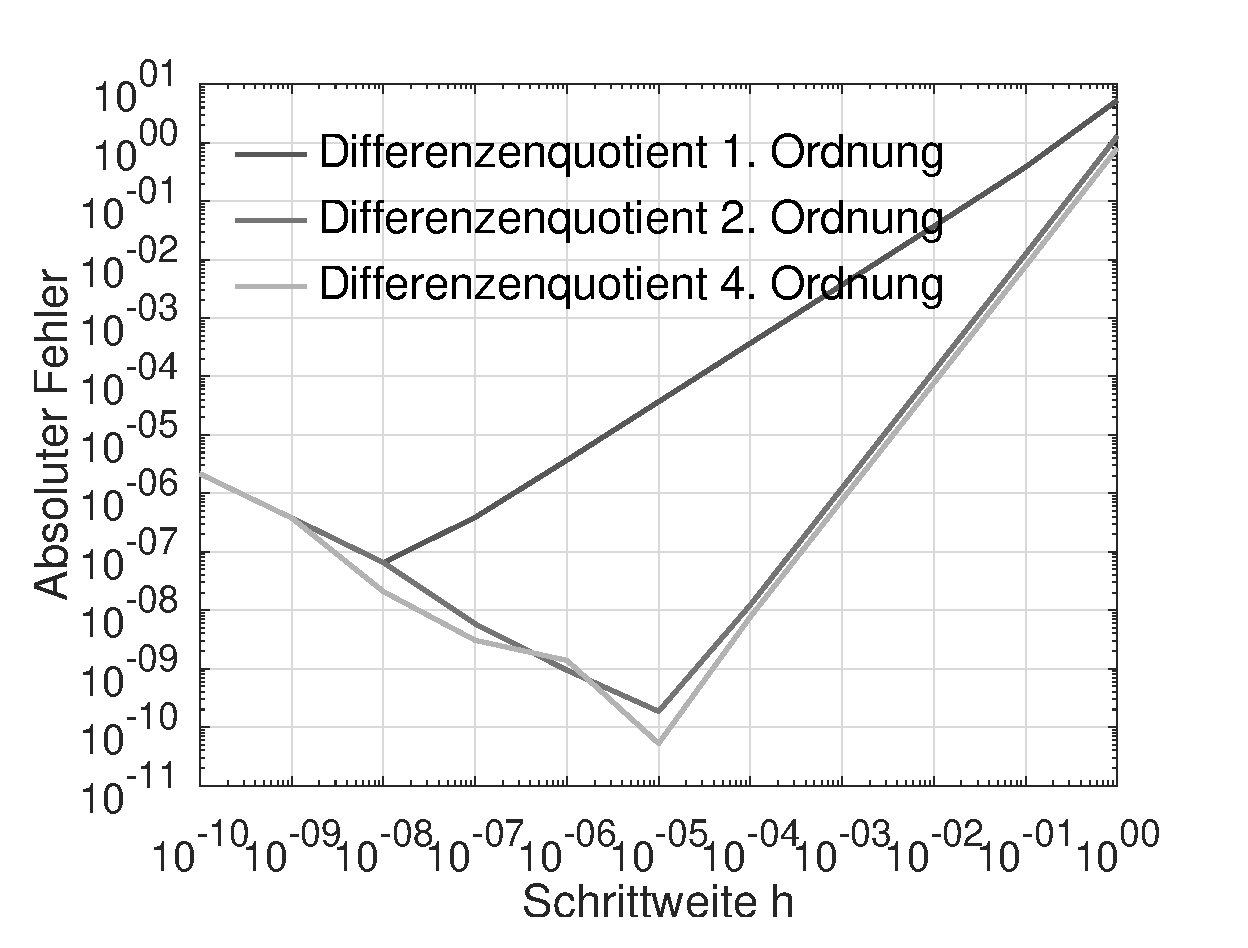
\includegraphics[width=\textwidth]{data/eFunktion}
		\caption{Fehler bei der Approximation von $f(x) = \exp(x+1)$ an der Stelle $x=1$}
		\label{fig:eFunktion}
	\end{subfigure}
	\begin{subfigure}[tpbh]{0.68\textwidth}
		\centering
		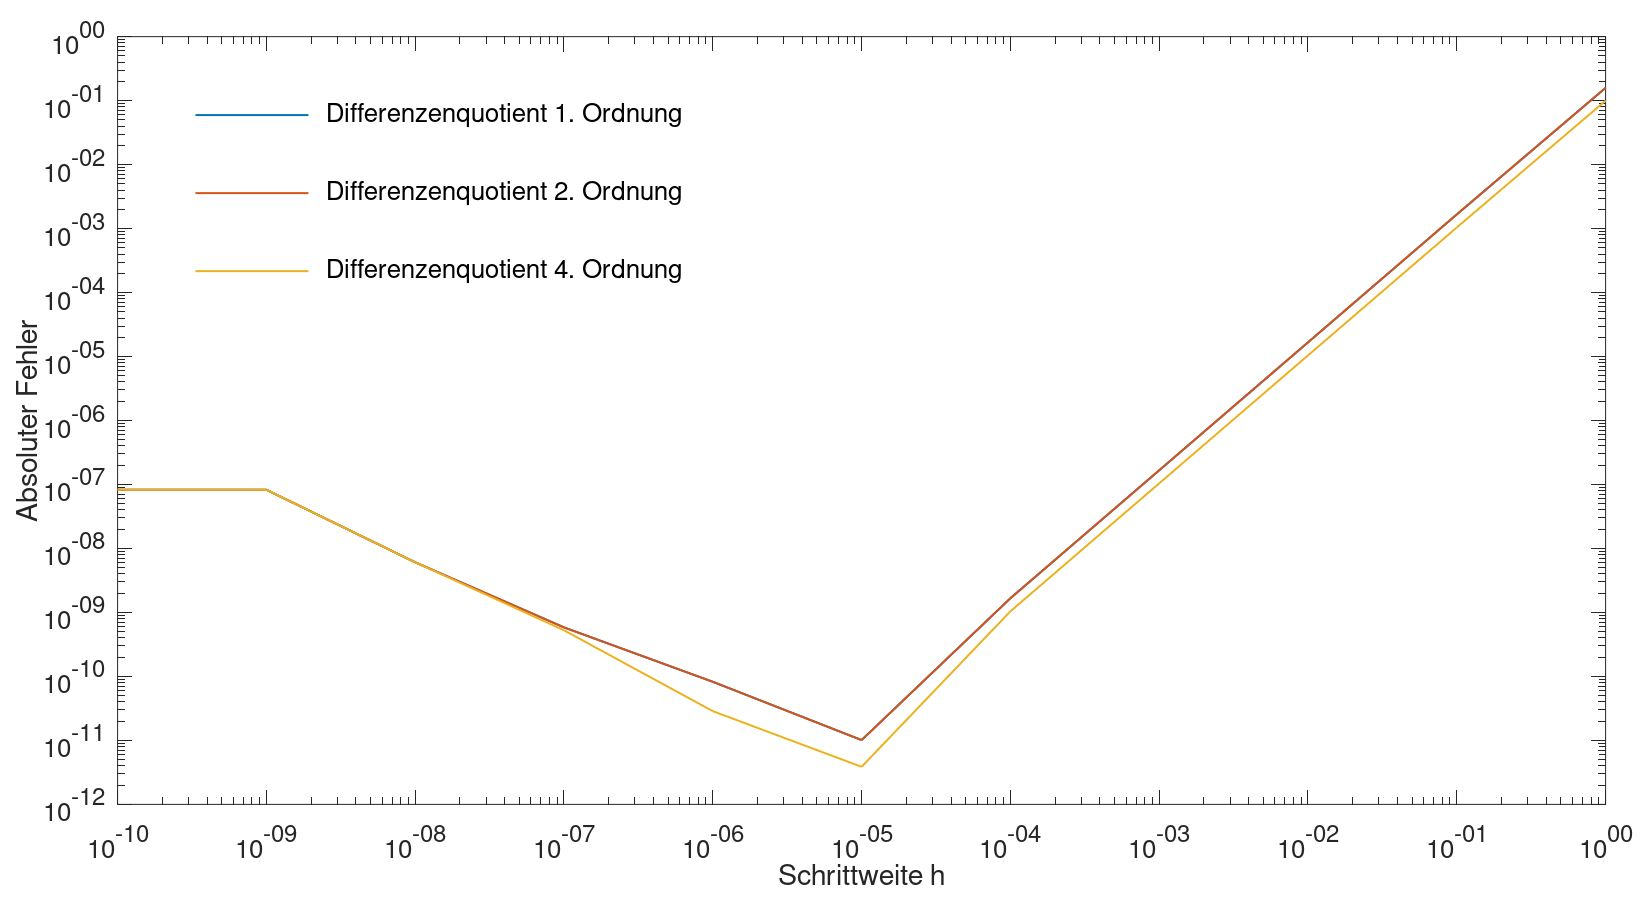
\includegraphics[width=\textwidth]{data/sinus}
		\caption{Fehler bei der Approximation von $g(x) = \cos(x)$ an der Stelle $x=\frac{\pi}{2}$}
		\label{fig:cosinus}
	\end{subfigure}
	\begin{subfigure}[tpbh]{0.68\textwidth}
		\centering
		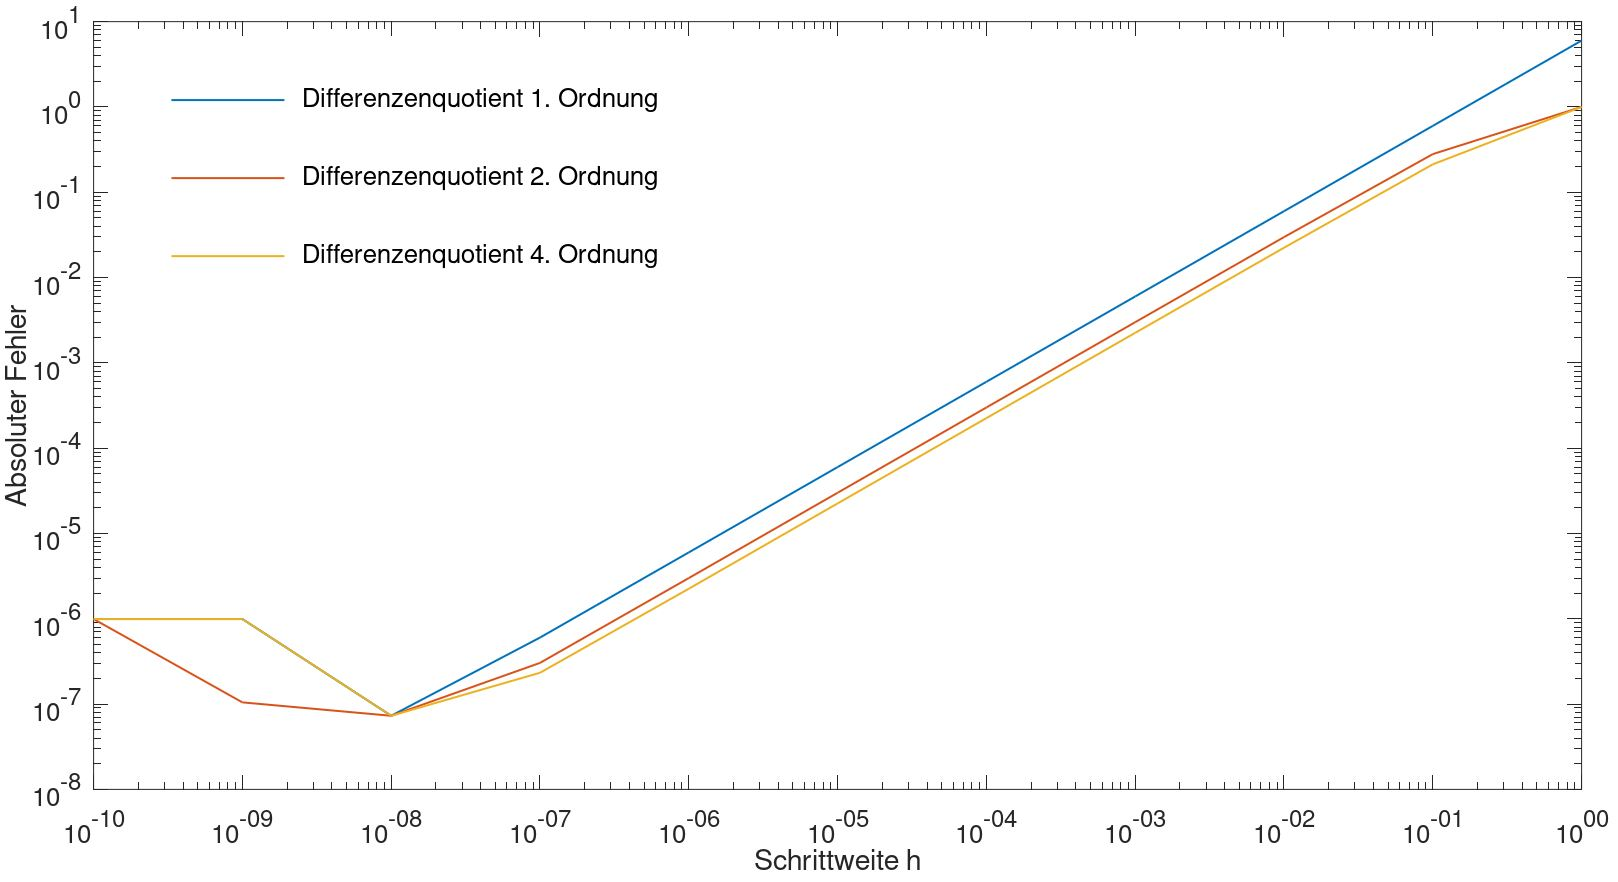
\includegraphics[width=\textwidth]{data/abschnittsFkt}
		\caption{Fehler bei der Approximation von (\ref{polynom}) an der Stelle $x=1$ }
		\label{fig:Polynom}
	\end{subfigure}
	\caption{Fehler der numerischen Approximationen der ersten Ableitung im doppelt logarithmischen Koordinatensystem}
	\label{fig:fehlerPlots}
\end{figure}



Um in einem doppelt logarithmischem Koordinatensystem die Steigung einer Geraden zu berechnen (siehe Abbildung \ref{steigung}), reicht es nicht wie bei einem linearen Koordinatensystem die Werte $\Delta x$ und $\Delta y$ des allgemeinen Steigungsdreiecks durch die Differenz der auf den Achsen angegebenen Werte zu ermitteln.\\
Stattdessen wird auf die Werte, die man an den jeweiligen Stellen auf den Achsen ablesen kann, der Logarithmus zur selben Basis angewandt, der zur Erzeugung der logarithmischen Skala verwendet wurde. In diesem Beispiel zur Basis $10$. Der Quotient zur Ermittlung der Steigung lautet dann 

\begin{equation*}
	\frac{\Delta y}{\Delta x} = \frac{\log(C (10^{\Delta r +r})^p)-\log(C (10^r)^p)}{\log(10^{\Delta r +r}) - \log(10^r)}
\end{equation*} 

und unter Anwendung der Logarithmus Regeln $\log(u\cdot v) = \log u + \log v$ und $\log (10^w) = w$ folgt

\begin{equation*}
	\frac{\Delta y}{\Delta x} = \frac{(p(\Delta r +r)-pr)}{r+\Delta r -r}
	=p.
\end{equation*}

Die Steigung der Fehlerabschätzung $\epsilon (h)$ ist somit genau gleich mit der Ordnung $p$ des jeweiligen numerischen Verfahrens zur Approximation.

\begin{figure}[htpb]
	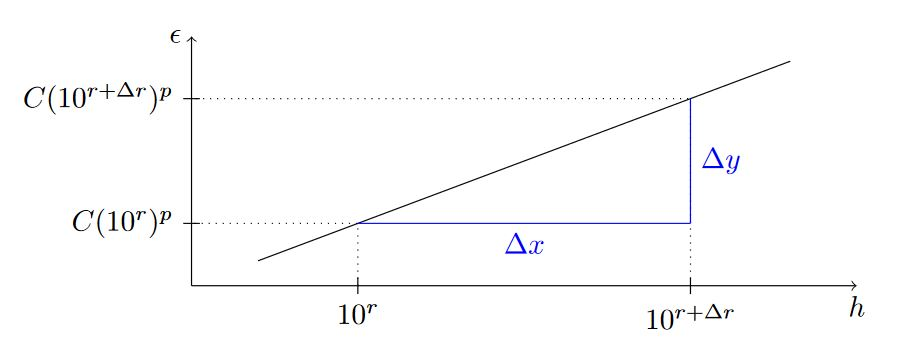
\includegraphics[width=\textwidth]{data/SteigungLogPlot}
	\caption{Allgemeines Steigungsdreieck in einem doppelt Logarithmischen Koordinatensystem}
	\label{steigung}
\end{figure}

Hat das logarithmische Koordinatensystem nicht die Basis 10, sondern eine beliebige andere, ist die Steigung für $\epsilon (h)$ weiterhin durch die Ordnung $p$ gegeben. Zur Berechnung des allgemeinen Steigungsdreiecks wird, wie bereits beschrieben, der Logarithmus zur selben beliebigen Basis auf alle Werte angewendet, somit ist die Basis des Logarithmus unerheblich für die Steigung.






	\section{Implizites Euler Verfahren}\label{sec:ag4_2}




	\section{Numerische Lösung linearer Gleichungssysteme}
Bei numerischen Berechnungen spielen lineare Gleichungssysteme der Form \textbf{Ax}=\textbf{y} oft eine überaus wichtige Rolle. Daher ist es sinnvoll und von Nöten effiziente Lösungsverfahren für diese Gleichungssysteme zu entwickeln und anzuwenden. In diesem Abschnitt werden verschiedene Verfahren in Octave implementiert und an beispielhaften Gleichungssystemen getestet und gegeneinander verglichen.\\ \\
Zunächst wird eine vorgegebene quadratische Matrix betrachtet. Mit Hilfe des Befehls \texttt{spy} lassen sich Matrizen in Octave graphisch darstellen. In Abb. \ref{fig:bspMat} ist diese Graphik zu sehen, die blauen Punkte in dem Plot sind Einträge, die ungleich null sind. Zählt man diese mit dem Befehl \texttt{nnz} findet man heraus, dass 3678 der 158404 Einträge ungleich null sind. Weiterhin lässt sich aus der Abbildung und der Darstellung der Werte in Octave herausfinden, dass es sich um eine symmetrische Matrix handelt, das heißt die Einträge der Matrix sind spiegelsymmetrisch bezüglich der Hauptdiagonalen. \\ \\
\begin{figure}[h]
	\begin{subfigure}[c]{.48\textwidth}
		\centering
		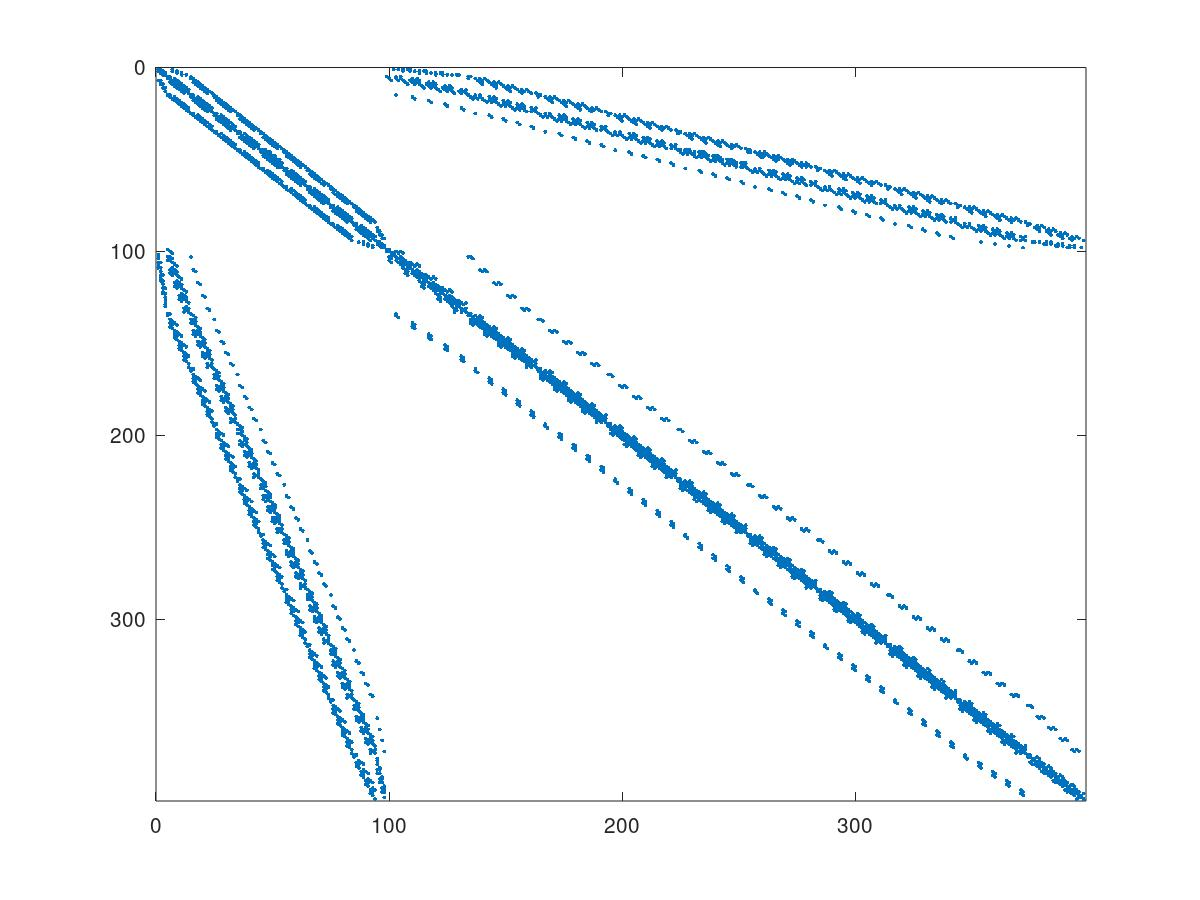
\includegraphics[width=\textwidth]{data/MatrixBsp}
		\subcaption{Graphische Darstellung der mit Octave eingelesene Beispielmatrix}
		\label{fig:bspMat}
	\end{subfigure}
	\begin{subfigure}[c]{.48\textwidth}
		\centering
		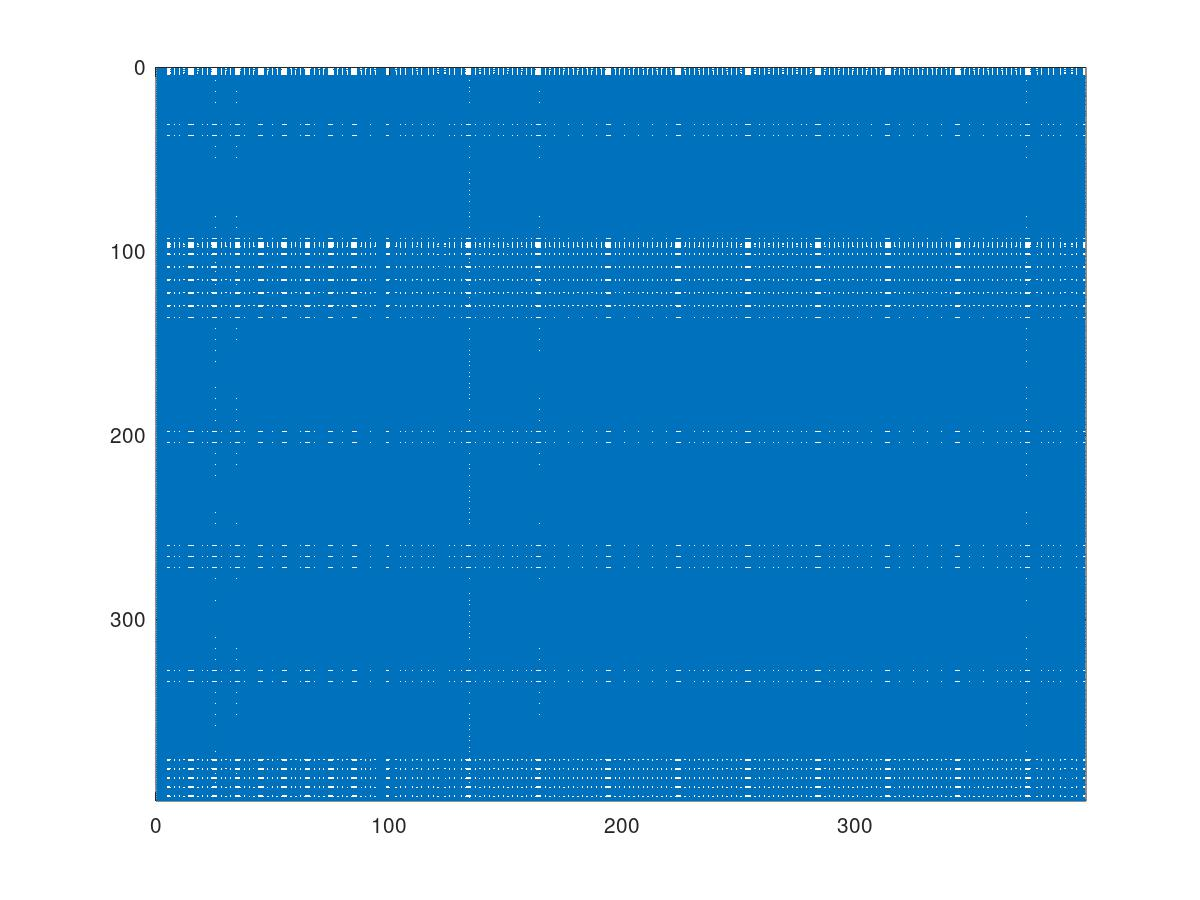
\includegraphics[width=\textwidth]{data/MatrixInv}
		\subcaption{Berechnete Inverse der eingelesenen Matrix}
		\label{fig:inv}\vspace{12pt}
	\end{subfigure}
	\caption{Graphische Darstellung von Matrizen, die blauen Punkte stellen Einträge dar, die ungleich null sind}
\end{figure} \\ 
Nun soll ein erstes Lösungsverfahren in Octave implementiert werden. Das \textsc{Gauss
'sche}-Eliminationsverfahren wurde in Listing \ref{lst:Elim} implementiert. Die Routine \texttt{gaussElim} erhält einen stehenden Vektor \textbf{b} mit Länge $n$ und eine quadratische Matrix \textbf{A} der Größe $n \times n$. Die Rückgabe ist ein Vektor \textbf{x} mit Länge $n$, der die berechneten Lösungen $x_{1}, \dots, x_{n}$ unseres linearen Gleichungssystems enthält.\\ \\
Zunächst wird \texttt{n}, also die Größe der Matrix bestimmt, daraufhin wird der Ergebnisvektor \textbf{x} mit entsprechender Länge erzeugt. In Zeile 4 und 5 werden zwei Laufvariablen initialisiert, \texttt{j} läuft hierbei über die Spalten, \texttt{i} über die Zeilen. Das Ziel des Algorithmus ist es schrittweise aus der übergebenen Matrix eine untere Dreiecksmatrix zu erstellen. Hierzu werden sogenannte Eliminationsfaktoren bestimmt, siehe Listing \ref{lst:Elim} Zeile 6. Mit Hilfe einer weiteren Laufvariable \texttt{k}, die über die Spalten von \texttt{j} bis \texttt{n} läuft. In der Schleife, Zeile 7 bis 9, werden Zeilenadditionen durchgeführt, um so Spalte für Spalte Nulleinträge zu erzeugen. Auch der Vektor \textbf{b} wird entsprechend angepasst. \\
In den Zeilen 14 bis 17 wird das Gleichungssystem final gelöst, die einzelnen $x_{1}, \dots, x_{n}$ werden von unten nach oben mit Hilfe der Matrix und dem Vektor \textbf{b} berechnet.  \\
Durch die drei ineinander geschachtelten For-Schleifen in den Zeilen 4 bis 12 erhalten wir eine kubische Anzahl an Rechenschritten, $n^{3}-n^{2}$, Zeile 14 bis 17 führen zu einem zusätzlichen Rechenaufwand von $n^{2}-n$, daraus ergibt sich die Abschätzung $\mathcal{O}(n^{3})$.
\lstinputlisting[label=lst:Elim,numbers=left]{data/gaussElim.m} 
Lineare Gleichungssysteme lassen sich auch mit Hilfe der Inversen einer Matrix bestimmen. In Octave geht dies mit dem Befehl \texttt{inv(A)}. Wie aus Abbildung \ref{fig:inv}, verglichen mit Abbildung \ref{fig:bspMat}, hervorgeht, hat die Invertierte Matrix deutlich mehr Einträge, die ungleich null sind. Die Berechnung der Inversen benötigt sehr viel Arbeitsspeicher und es werden deutlich mehr Rechenoperationen ausgeführt, um die Lösungen zu berechnen.\\ \\

%%%%%%%%%%%%%%%%%%%%%%%%% Aufgabenteil d %%%%%%%%%%%%%%%%%%%%%%%%%%%%
Eine weitere Methode mit der lineare Gleichungssysteme effizient berechnet werden können ist die LUPQ-Zerlegung. Bei der LUPQ-Zerlegung wird die Matrix \textbf{A} mit Hilfe des bereits vorgestellten \textsc{Gauss'schen}-Eliminationsverfahren in eine obere und eine untere Dreiecksmatrizen aufgeteilt, es gilt $\textbf{A} = \textbf{L} \textbf{U}$. Mit Hilfe von Vorwärts-/Rückwärtseinsetzen lässt sich nun das Gleichungssystem lösen. Zum Lösen wird zunächst vorwärts $$ \textbf{Ly} = \textbf{b}$$ eingesetzt und anschließend rückwärts $$ \textbf{Ux} = \textbf{y}$$ berechnet. Zum berechnen unterschiedlicher Seiten \textbf{b} muss die Matrix nicht neu zerlegt, sondern nur das Vorwärts-/Rückwärtseinsetzen betrachtet werden. Auch dieses Verfahren ist in Octave bereits vorimplementiert und lässt sich mit dem Befehl \texttt{lu(A)} aufrufen. Es ergeben sich bei dieser Methode Unterschiede, die durch die Anzahl der zur Verfügung gestellten Variable in denen die Lösung gespeichert werden soll, hervorgerufen werden.\\
Gibt man der Methode zwei Variablen zum Speichern der Ergebnisse vor, so entsteht nicht wie erwartet eine obere und eine untere Dreiecksmatrix, sondern die in Abbildung \ref{fig:LLU} zu sehende Matrix \textbf{L} und die in Abb. \ref{fig:ULU} Matrix \textbf{U}. Stellt man der Routine vier Variablen \texttt{[L, U, P, Q]} zum Speichern zur Verfügung so entsteht wie in Abb. \ref{fig:LLUPQ} und \ref{fig:ULUPQ} zu sehen ist jeweils eine obere und untere Dreiecks Matrix. Zudem haben diese Matrizen deutlich weniger Einträge. \textbf{P} ist eine Permutationsmatrix. Mit dieser werden Zeilen und Spalten der Ausgangsmatrix \textbf{A} vertauscht, um zu kleine Pivot Elemente, die zu großen Rundungsfehlern führen können, zu verhindern und zu garantieren, dass die Zerlegung in eine obere und untere Dreiecksmatrix möglich ist. 

\begin{figure}[h!]
	\begin{subfigure}[h]{.48\textwidth}
		\centering
		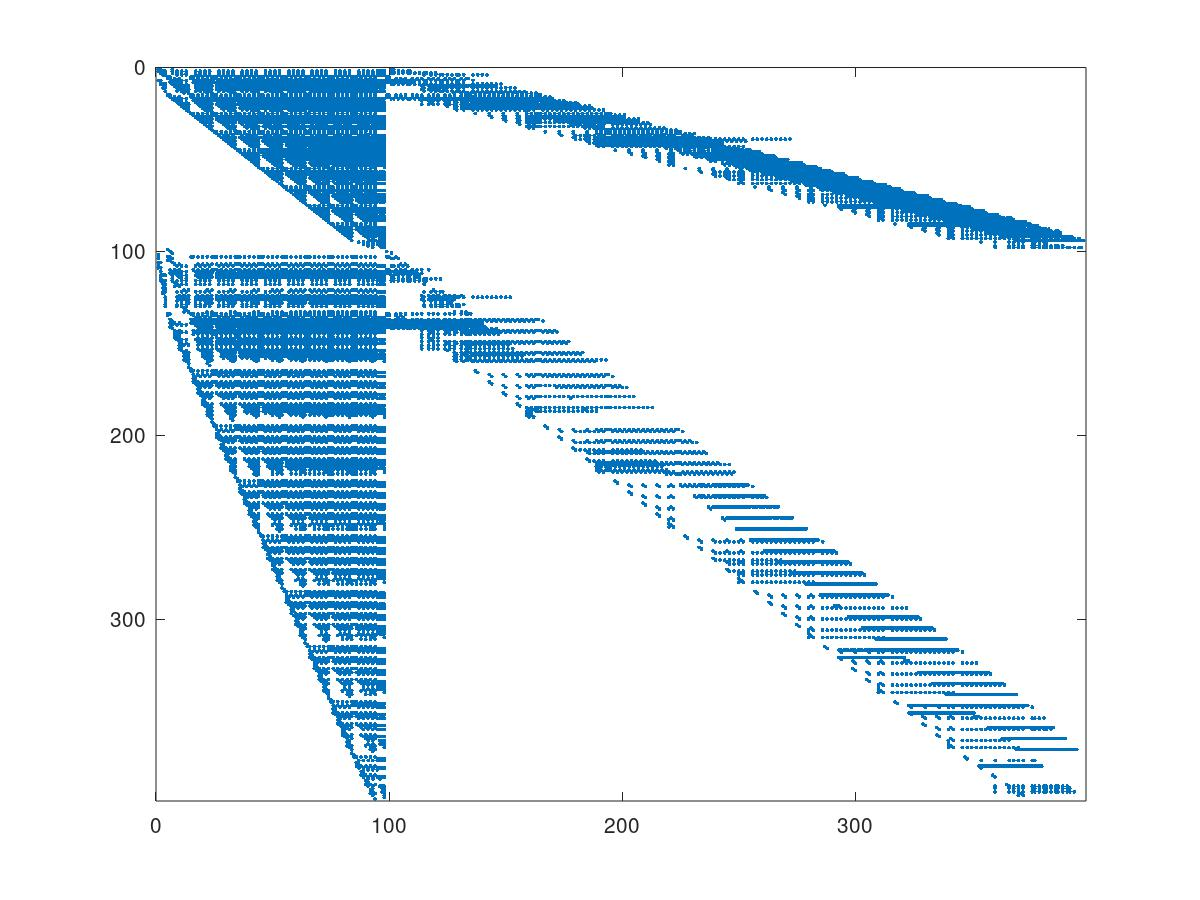
\includegraphics[width=\textwidth]{data/LLU}
		\subcaption{Matrix \textbf{L} nach LU-Zerlegung}
		\label{fig:LLU}
	\end{subfigure}
	\begin{subfigure}[h]{.48\textwidth}
		\centering
		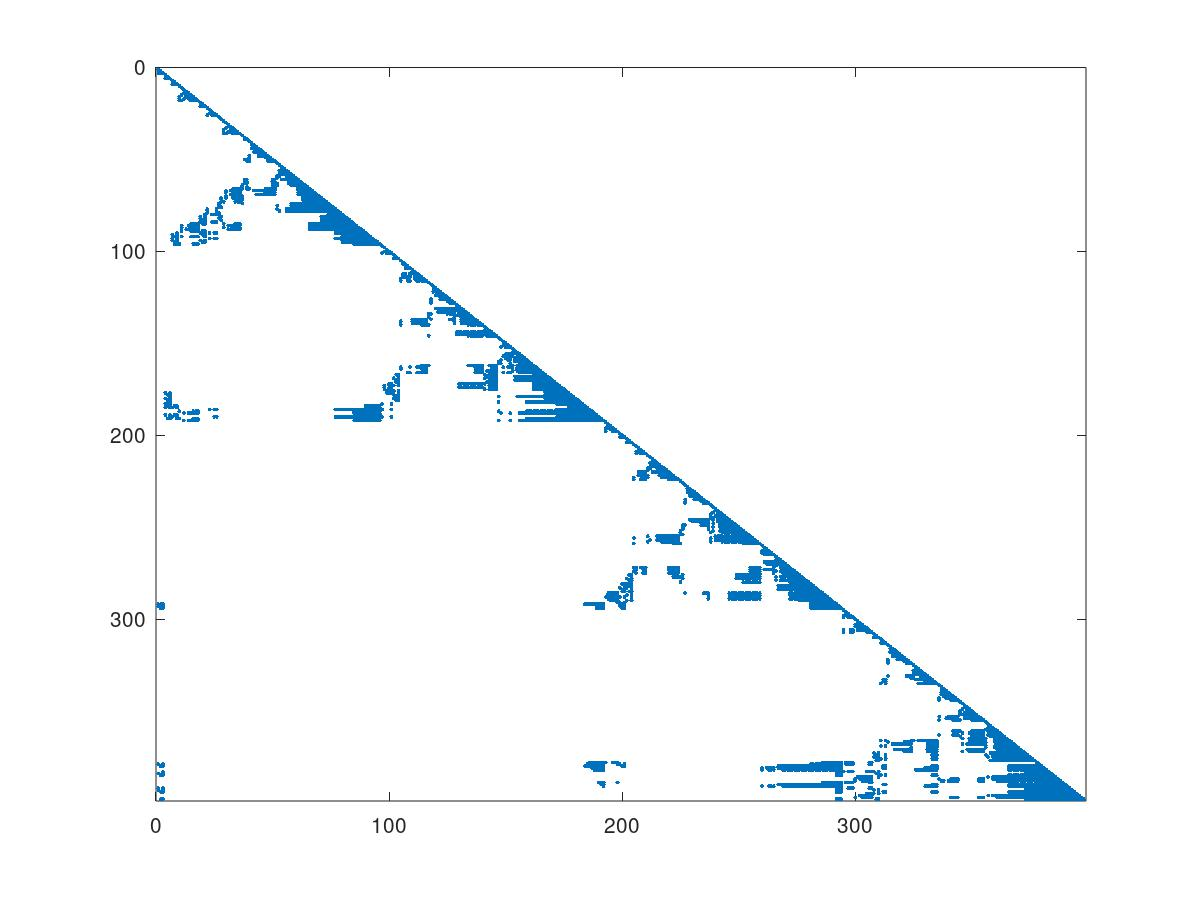
\includegraphics[width=\textwidth]{data/LLUPQ}
		\subcaption{Matrix \textbf{L} nach LUPQ-Zerlegung}
		\label{fig:LLUPQ}
	\end{subfigure}
	\begin{subfigure}[h]{.48\textwidth}
		\centering
		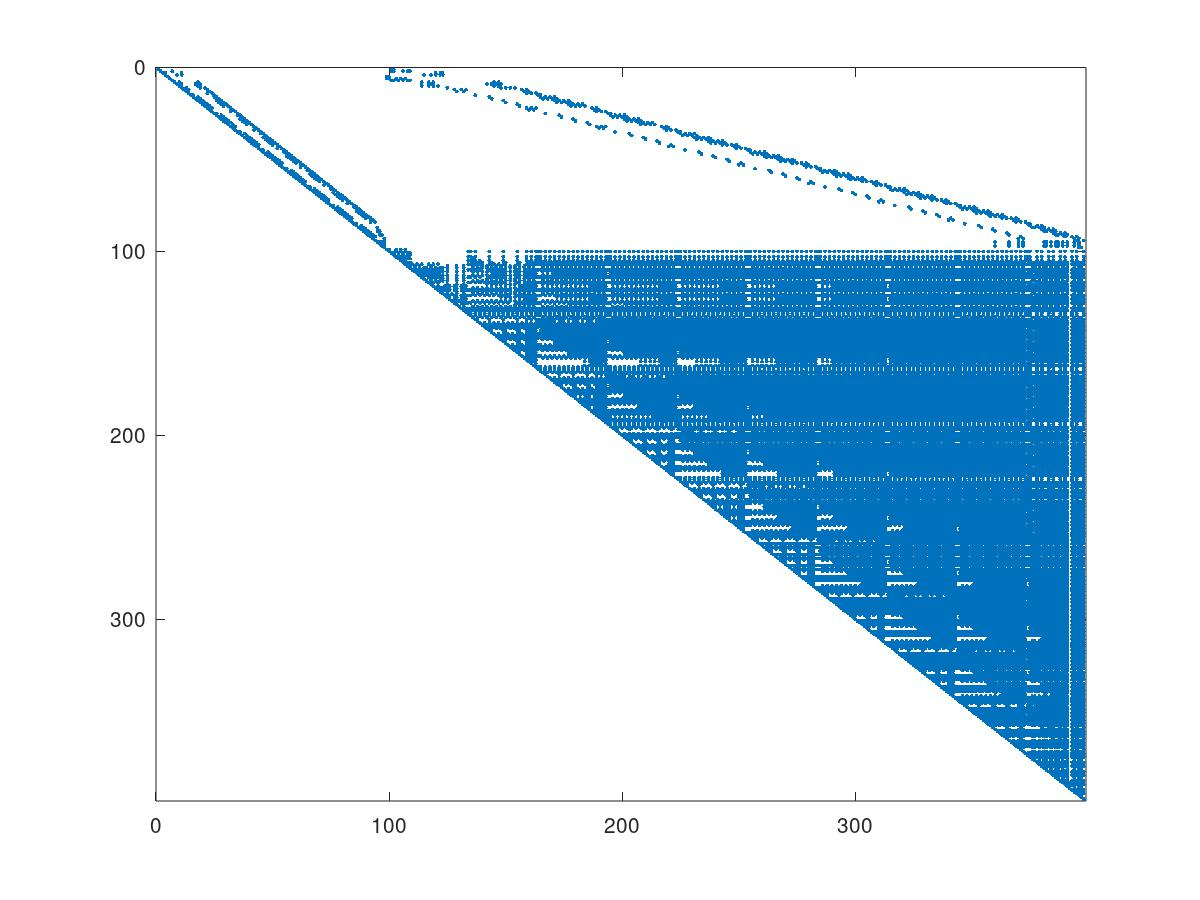
\includegraphics[width=\textwidth]{data/ULU}
		\subcaption{Matrix \textbf{U} nach LU-Zerlegung}
		\label{fig:ULU}
	\end{subfigure}
	\begin{subfigure}[h]{.48\textwidth}
		\centering
		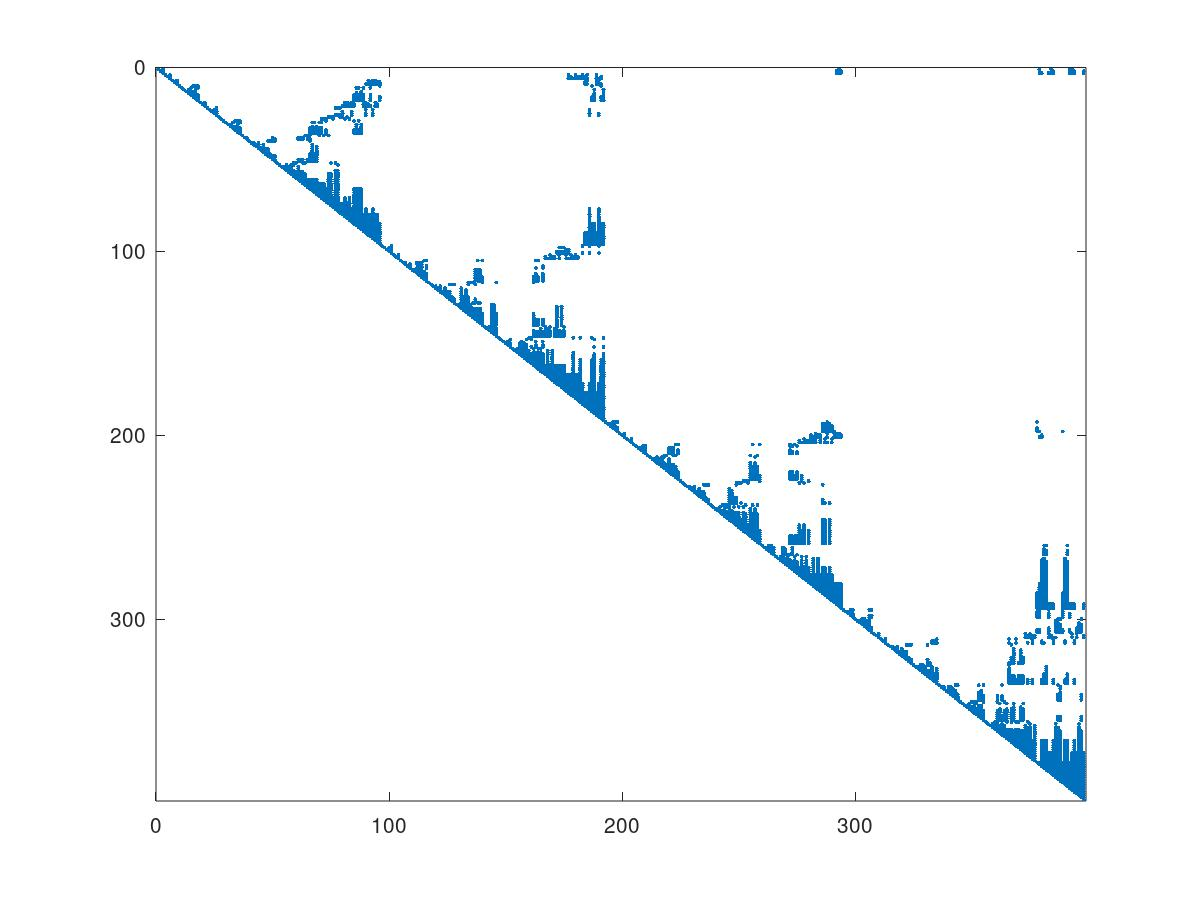
\includegraphics[width=\textwidth,]{data/ULUPQ}
		\subcaption{Matrix \textbf{U} nach LUPQ-Zerlegung}
		\label{fig:ULUPQ}
	\end{subfigure}\hspace{40pt}
\caption{Darstellung der unterschiedlichen Matrizen, die abhängig der zur Verfügung gestellten Lösungsvariablen entstehen}
\end{figure}
Um den zeitlichen Aufwand der einzelnen Lösungsverfahren besser vergleichen zu können wird im Folgenden eine Messung der benötigten Rechenzeit in Octave durchgeführt und beschrieben. Die zu vergleichenden Lösungsverfahren zur Berechnung linearer Gleichungssysteme sind die LUPQ-Zerlegung, Lösung mit Hilfe des Backslash-Operators und die Berechnung mit der Inversen.\\ \\
Verschiedene tridiagonale Testmatrizen \textbf{A} der Größe $n \times n$ mit $n \in [500, 1000, 2000, 4000, 8000]$ haben jeweils 10 unterschiedliche, zufällige Seiten \textbf{b} zugewiesen bekommen. Die Zeit zur Berechnung jeder einzelnen Seite wurde gespeichert, die Berechnung der Inversen bzw. der LUPQ Zerlegung fließt nur bei der ersten Berechnung mit in die Rechenzeit ein. \\
Die Rechenzeit, die benötigt wurde um alle 10 Seiten zu berechnen wurde schließlich durch 10 geteilt, um eine durchschnittliche Rechenzeit zu erhalten. Die Ergebnisse wurden abschließend auf einem doppelt logarithmischen Koordinatensystem geplottet, wobei die x-Achse die Größe $n$ der Matrix ist und die y-Achse die zur Berechnung einer Seite benötigte Rechenzeit.
\begin{figure}
	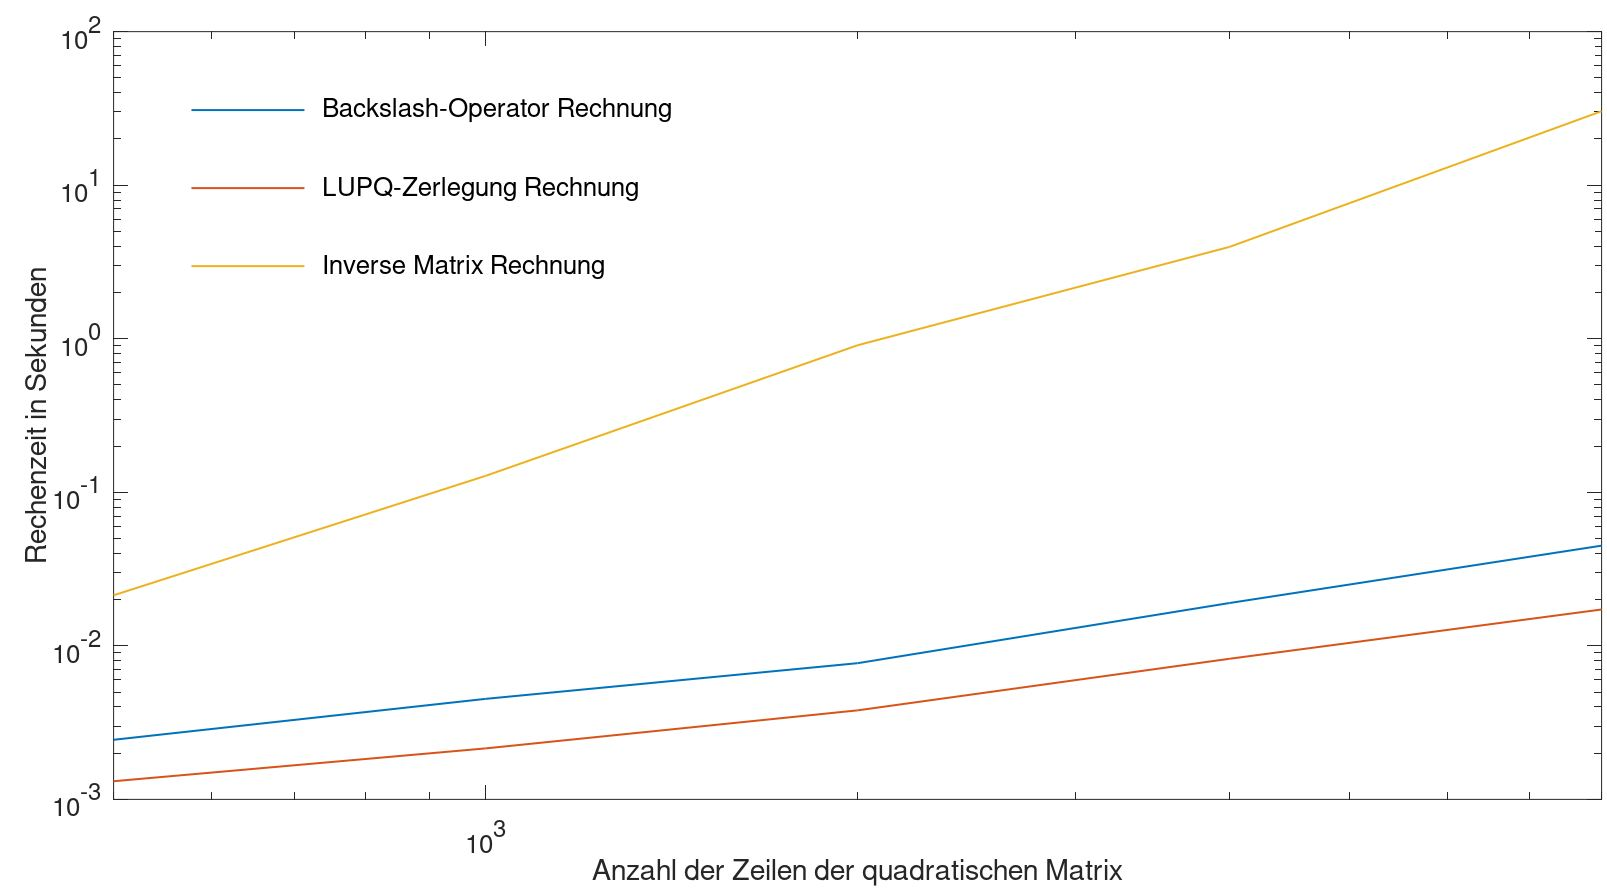
\includegraphics[width=\textwidth]{data/LaufzeitPlot}
	\caption{Graphische Darstellung der Rechenzeit, die unterschiedliche Lösungsverfahren zum Lösen linearer Gleichungen benötigen}
	\label{fig:Laufzeit}
\end{figure}
\\ \\
Wie aus Abbildung \ref{fig:Laufzeit} erkenntlich ist, benötigt die LUPQ-Zerlegung die geringste Zeit, um die Gleichungssysteme zu lösen. Der Backslash Operator benötigt mehr Zeit, ist aber, verglichen zur Berechnung mit Hilfe der Inversen, immer noch effizient. 
	
	%%%%%%%%%%%%%%%%%%Fazit%%%%%%%%%%%%%%%%%%%%%%
	\chapter{Fazit}\label{sec:fazit}
%\addcontentsline{toc}{section}{Fazit}
Die erste Aufgabe ergab, dass sich die beiden Leiter des Koaxialkabels wie die Platten eines Plattenkondensators verhalten. Darüber hinaus ergibt sich, dass man durch Anfügen von weiteren Segmenten an die Schaltung eine Verkleinerung der Schwingfrequenz bewirkt.
Differentialgleichungen können häufig, wie sich in Aufgabe zwei zeigt, leichter im Frequenzbereich als im Zeitbereich gelöst werden. Die durch Lösen der Differentialgleichung analytisch berechneten Ergebnisse für Zeit- und Frequenzverhalten stimmen dabei mit der numerischen Simulation durch LTSpice überein.
Die Ergebnisse der dritten Aufgabe ergeben, dass sich die Feldlinien eines Kondensators in einem Simulationskäfig nicht nur senkrecht zu den Platten bewegen, sondern dass sich auch Randeffekte an den Enden der Kondensatorplatten ausbilden. Untersucht man unterschiedliche Randbedingungen zeigt sich, dass diese sowohl den Kapazitätswert des Kondensators, als auch die elektrischen Feldlinien beeinträchtigen. Die Wahl der Simulationsrandbedingungen kann also nicht willkürlich erfolgen.
	%%%%%%%%%%%%%%%%%%Anhang%%%%%%%%%%%%%%%%%%%%%
	\chapter{Anhang}\label{sec:anhang}
\lstset{ % Octave Settings
	language=Octave,
	extendedchars=true,
	basicstyle=\footnotesize,
	numbers=left,
	numberstyle=\tiny\color{gray},
	stepnumber=1,
	numbersep=10pt,
	showspaces=false,
	showstringspaces=false,
	tabsize=2,
	breaklines=true,
	frame=single,
	morecomment = [l][\itshape\color{blue}]{\%},
	captionpos=b,
	title=\lstname
}


\lstinputlisting{data/SIS.m}
\lstinputlisting{data/SkriptAg8_2.m}
\lstinputlisting{data/SkriptAg8_3d.m}



	%%%%%%%%%%%%%%%%%%%%%%%%%%%%%%%%%%%%%%%%%%%%%%%%%%%%%%%%%%%%%%%%%%%%%%%%%%%%%%%%%%%%%%%%%%%%%%%%%%
	
	%%%%%%%%%%%%%%%%%%%
	%Abbildungs- und Tabellenverzeichnis
	%%%%%%%%%%%%%%%%%%%
	\listoffigures % Abbildungsverzeichnis (captions in den Figuren werden als Referenz genommen)
	%\listoftables % Verzeichnis der Tabellen (captions in den Tabellen werden als Referenz genommen)
	
	%%%%%%%%%%%%%%%%%%%
	%Literaturverzeichnis an dieser Stelle
	%%%%%%%%%%%%%%%%%%%
	
	
\end{document}
